\section{Evaluation}\seclabel{Evaluation}
In this section, we describe and evaluate Lucy: a prototype implementation of
our decision procedures and system models.

\subsection{Implementation}
Lucy includes an implementation of the interactive decision procedure described
in \algoref{InteractiveDecisionProcedure}, an implementation of a decision
procedure which checks criteria (1) - (4) from \thmref{LatticeProperty}, and an
implementation of the decision procedure described in
\algoref{ArbitraryStartInteractiveDecisionProcedure}. The decision procedures
are implemented in roughly 2,500 lines of Python. Users specify objects,
transactions, and invariants in a small Python DSL and interact with the
interactive decision procedures using an interactive Python console. We use
Z3~\cite{de2008z3} to implement our \invariantclosure{} decision procedure,
compiling an object and invariant into a formula that is satisfiable if and
only if the object is \emph{not} \invariantclosed{}. If the object is
\invariantclosed{}, then Z3 concludes that the formula is unsatisfiable.
Otherwise, if the object is not \invariantclosed{}, then Z3 produces a
counterexample witnessing the satisfiability of the formula.

Lucy also includes an implementation of the \invariantconfluence{} and
segmented-invariant confluence system models in roughly 3,500 lines of C++.
Users specify objects, transactions, invariants, and segmentations in C++. Lucy
then replicates the objects using segmented \invariantconfluence{}. Clients
send every transaction request to a randomly selected server. When a server
receives a transaction request, it executes \algoref{TxnExecution} to attempt
to execute the transaction locally.  If the transaction requires global
coordination, then the server forwards the transaction request to a
predetermined leader. When the leader receives a transaction request, it
broadcasts a coordination request to the other servers. When a server receives
a coordination request from the leader, it stops processing transactions and
sends the leader its state. When the leader receives the states of all other
servers, it executes the transaction, and then sends its state to the other
servers. When a server receives a new state, it adopts the state, computes its
new active segment, and resumes normal processing. After every 100 transactions
processed, a server sends a merge request to a randomly selected server.

Lucy can also replicate an object with eventual consistency and with
linearizability. With eventual consistency, clients send every transaction
request to a randomly selected server. The server executes the transaction
locally and returns immediately to the client, sending merge requests after
every 100 transactions. With linearizability, clients send every transaction
request to a predetermined leader. The leader relays the transaction request to
all other servers, and when the leader receives replies from them, it executes
the transaction and replies to the client. This communication pattern mimics
the ``normal operation'' of state machine replication protocols
\cite{lamport1998part, liskov2012viewstamped}.

Because fault-tolerance is largely an orthogonal concern to
\invariantconfluence{}, Lucy is implemented without fault-tolerance. It would
be straightforward to add fault-tolerance to Lucy, but it would not affect our
discussions or evaluation, so we leave it for future work.

\subsection{Decision Procedures}
We now evaluate the practicality and efficiency of our decision procedure
prototypes. We begin by demonstrating the decision procedure on a handful of
simple, yet practical examples. We then discuss how our tool can be used to
analyze the TPC-C benchmark. A summary of these results is given in
\tabref{EvalTable}.

{\begin{table}[t]
  \centering
  \caption{\exampleref{TwoIntsEval} to \exampleref{TpccEval} Summary}%
  \tablabel{EvalTable}
  \begin{tabular}{lrr}
    \toprule
    Example                                          & Run time (s) & Lines of code \\\midrule
    \ref{exa:TwoIntsEval}                            & 0.09         & 7 \\
    \ref{exa:ForeignKeysEval} (all transactions)     & 0.06         & 8 \\
    \ref{exa:ForeignKeysEval} (limited transactions) & 0.09         & 10 \\
    \ref{exa:AuctionEval}                            & 0.04         & 21 \\
    \ref{exa:EscrowTransactionsEval}                 & 0.09         & 49 \\
    \ref{exa:TpccEval} (Invariant 1)                 & 0.46         & 66 \\
    \ref{exa:TpccEval} (Invariant 2)                 & 0.44         & 33 \\
    \bottomrule
  \end{tabular}
\end{table}
}

\example[$\ints^2$]\examplelabel{TwoIntsEval}
We begin with a minimal working example. Consider again our recurring example
of $\ints^2$ from \exampleref{Z2}. The Python code used to describe the object,
transactions, and invariant is given in \figref{Z2Code}. When we call
\python{checker.check()}, the interactive decision procedure produces a
counterexample $s_1 = (0, 1), s_2 = (1, 0)$ in less than a tenth of a second
and automatically recognizes that $s_2$ is reachable. After we label $s_1$ as
unreachable and refine the invariant with $y \leq 0$, the interactive decision
procedure determines that the object is \invariantconfluent{}, again, in less
than a tenth of a second. Note that the object is \invariantconfluent{} but
\emph{not} \invariantclosed{}, so prior work~\cite{li2012making,
li2014automating, balegas2015towards, gotsman2016cause} that relies on
\invariantclosure{}---or another equivalent sufficient condition---to determine
\invariantconfluence{} would not be able to identify this example as
\invariantconfluent{}.

\begin{figure}[ht]
  \begin{Python}[gobble=4]
    checker = InteractiveInvariantConfluenceChecker()
    x = checker.int_max('x', 0) # An int, x, merged by max.
    y = checker.int_max('y', 0) # An int, y, merged by max.
    checker.add_transaction('increment_x', [x.assign(x + 1)])
    checker.add_transaction('decrement_y', [y.assign(y - 1)])
    checker.add_invariant(x * y <= 0)
    checker.check()
  \end{Python}
  \caption{\exampleref{TwoIntsEval} specification}\figlabel{Z2Code}
\end{figure}

\example[Foreign Keys]\examplelabel{ForeignKeysEval}
A 2P-Set $X = (A_X, R_X)$ is a set CRDT composed of a set of additions $A_X$
and a set of removals $R_X$~\cite{shapiro2011comprehensive}. We view the state
of the set $X$ as the difference $A_X - R_X$ of the addition and removal sets.
To add an element $x$ to the set, we add $x$ to $A_X$. Similarly, to remove $x$
from the set, we add it to $R_X$. The merge of two 2P-sets is a pairwise union
(i.e. $(A_X, R_X) \join (A_Y, R_Y) = (A_X \cup A_Y, R_X \cup R_Y)$).

We can use 2P-sets to model a simple relational database with foreign key
constraints. Let object $O = (X, Y) = ((A_X, R_X), (A_Y, R_Y))$ consist of a
pair of two 2P-Sets $X$ and $Y$, which we view as relations. Our invariant $X
\subseteq Y$ (i.e. $(A_X - R_X) \subseteq (A_Y - R_Y)$) models a foreign key
constraint from $X$ to $Y$. We ran our decision procedure on the object with
initial state $((\emptyset, \emptyset), (\emptyset, \emptyset))$ and with
transactions that allow arbitrary insertions and deletions into $X$ and $Y$.
After less than a tenth of a second, the decision procedure produced a
reachable counterexample witnessing the fact that the object is not
\invariantconfluent{}. A concurrent insertion into $X$ and deletion from $Y$
can lead to a state that violates the invariant. This object is not
\invariantconfluent{} and therefore not \invariantclosed{}. Thus, previous
tools depending on \invariantclosure{} as a sufficient condition would be
unable to conclude definitively that the object is \emph{not}
\invariantconfluent{}.

We also reran the decision procedure, but this time with insertions into $X$
and deletions from $Y$ disallowed. In less than a tenth of a second, the
decision procedure correctly deduced that the object is now
\invariantconfluent{}. These results were manually proven
in~\cite{bailis2014coordination}, but our tool was able to confirm them
automatically in a negligible amount of time.

\example[Auction]\examplelabel{AuctionEval}
We now consider a simple auction system introduced in~\cite{gotsman2016cause}.
Our object consists of a set $B$ of integer-valued bids and a optional winning
bid $w$. Initially, $B = \emptyset$ and $w = \bot$ (indicating that there is no
winning bid yet) and we merge states by taking the union of $B$ and the maximum
of $w$ (where $\bot < n$ for all integers $n$). One transaction $t_b$ places a
bid $b$ by inserting it into $B$. Another transaction $t_\text{close}$ closes
the auction and sets $w$ equal to the largest bid in $B$. Our invariant is that
if the auction is closed (i.e.\ $w \neq \bot$), then $w = \max(B)$. We ran our
decision procedure on this example and in a third of a second, it produced a
reachable counterexample witnessing the fact that the object is not
\invariantconfluent{}.  If we concurrently close the auction and place a large
bid, then we can end up in a state in which the auction is closed, but there is
a bid in $B$ larger than $w$.

We then segmented our object as follows. The first segment $(\setst{(B, w)}{w =
\bot}, \setst{t_b}{b \in \ints})$ allows bidding so long as the bid is open.
The second segment $(\setst{B, w}{w \neq \bot} \cap I, \emptyset)$ includes all
auctions that have already been closed and forbids all transactions. This
segmentation captures the intuition that bids should be permitted only when the
auction is open. We ran our segmented \invariantconfluence{} decision procedure
on this example, and it was able to deduce without any human interaction that
the example was segmented \invariantconfluent{} in less than a tenth of a
second.

\example[Escrow Transactions]\examplelabel{EscrowTransactionsEval}
Escrow transactions are a concurrency control technique that allows a database
to execute transactions that increment and decrement numeric values with more
concurrency than is otherwise possible with general-purpose techniques like
two-phase locking~\cite{o1986escrow}. The main idea is that a portion of the
numeric value is put in escrow, after which a transaction can freely decrement
the value so long as it is not decremented by more than the amount that has
been escrowed. We show how segmented \invariantconfluence{} can be used to
implement escrow transactions.

Consider again the PN-Counter $s = (p_1, p_2, p_3), (n_1, n_2, n_3)$ from
\exampleref{CounreachableExample} replicated on three servers with transactions
to increment and decrement the PN-Counter. In
\exampleref{CounreachableExample}, we found that concurrent decrements violate
\invariantconfluence{} which led us to a segmentation which prohibited
concurrent decrements. We now propose a new segmentation with escrow amount $k$
that will allow us to perform concurrent decrements that respect the escrowed
value. The first segment $(\setst{(p_1, p_2, p_3), (n_1, n_2, n_3)}{p_1, p_2,
p_3 \geq k \land n_1, n_2, n_3 \leq k}, T)$ allows for concurrent increments
and decrements so long as every $p_i \geq k$ and every $n_i \leq k$.
Intuitively, this segment represents the situation in which every server has
escrowed a value of $k$. They can decrement freely, so long as they don't
exceed their escrow budget of $k$. The second segment is the one presented in
\exampleref{CounreachableExample} which prohibits concurrent decrements. We ran
our decision procedure on this example and it concluded that it was segmented
\invariantconfluent{} in less than a tenth of a second and without any human
interaction.

\example[TPC-C]\examplelabel{TpccEval}
TPC-C is a ubiquitous OLTP database benchmark with a workload that models a
simple warehousing application~\cite{difallah2013oltp}. The TPC-C specification
outlines twelve ``consistency requirements'' (read invariants) that govern the
warehousing application. In~\cite{bailis2014coordination}, Bailis et al.\
categorize the invariants into one of three types:

% \begin{enumerate}
%   \item
    Three of the twelve invariants are \textbf{foreign key constraints}.  As
    discussed in \exampleref{ForeignKeysEval}, our decision procedures can
    automatically verify conditions under which foreign key constraints are
    \invariantconfluent{}.

  % \item
    \newcommand{\ttt}[1]{{\smaller \texttt{#1}}} Seven of the twelve invariants
    involve \textbf{maintaining arithmetic relationships between relations}.
    Our decision procedures can correctly identify these as
    \invariantconfluent{}. Consider, for example, invariant 1 which dictates
    that a warehouse's year to date balance \ttt{W\_YTD} is equal to the sum of
    the district year to date balances \ttt{D\_YTD} of the twenty districts
    that are associated with the warehouse. The Payment transaction randomly
    selects a district and increments \ttt{W\_YTD} and \ttt{D\_YTD} by a
    randomly generated amount. We model this workload with a PN-Counter for
    \ttt{W\_YTD} and twenty PN-Counters for the twenty instances of
    \ttt{D\_YTD}. We applied Lucy to this workload, and it determined that the
    workload was \invariantconfluent{} in less than a second.

  % \item
    Two of the twelve invariants involve generating \textbf{sequential and
    unique identifiers}. Consider, for example, invariant 2 which dictates that
    a district's next order id \ttt{D\_NEXT\_O\_ID} is equal to the maximum
    order id \ttt{O\_ID} of orders within the district. The New Order
    transaction places an order with \ttt{O\_ID} equal to the current value of
    \ttt{D\_NEXT\_O\_ID} and then increments \ttt{D\_NEXT\_O\_ID}.
    We model this workload with an integer for \ttt{D\_NEXT\_O\_ID} and a map
    for \ttt{O\_ID} that maps order ids to order.
    %
    % We model this workload with three objects. \ttt{D\_NEXT\_O\_ID} is modeled
    % as an integer merged by $\max$. The order table is modelled as two objects.
    % The first is a set of all order ids used, merged by union. The second is a
    % map which maps order id to order. The map's merge function performs an
    % id-by-id merge of orders. If two different orders have the same id, the
    % merge function replaces them with a distinguished value to indicate that
    % the primary key constraint has been violated.
    %
    We applied Lucy to this workload and in less than a second, it produced a
    counterexample that---when labelled as reachable---confirms that the
    workload is \emph{not} \invariantconfluent{}~\cite{bailis2014coordination}.
% \end{enumerate}

\subsection{Segmented Invariant Confluence}%
\seclabel{SegmentedInvariantConfluenceEval}
Now, we evaluate the performance of replicating an object with segmented
\invariantconfluence{} as compared to the performance of replicating it with
eventual consistency or linearizability.
%
There are two hypotheses about the performance of segmented
\invariantconfluent{} replication that we aim to confirm.
%
First, segmented \invariantconfluent{} replication provides higher throughput
and better scalability than linearizable replication for workloads that
require little coordination (i.e.\ low-coordination workloads).
%
Second, the throughput and scalability of segmented \invariantconfluent{}
replication decreases as we increase the fraction of transactions that require
coordination.

These hypotheses state that segmented \invariantconfluent{} is more performant
than linearizable replication for low-coordination workloads. But by how much?
We also aim to measure the absolute performance and scalability benefits of
segmented \invariantconfluent{} replication and how they vary as we vary the
coordination required by a workload. We perform two controlled microbenchmarks
to confirm our hypotheses and discover the absolute performance benefits. The
workloads themselves are trivial, but also not salient. \jmh{Salient to what? I'm confused by the last sentence.} Our objective is to
obtain a controlled measure of throughput and scalability as we vary workload
contention.

\begin{figure}[t]
  \centering
  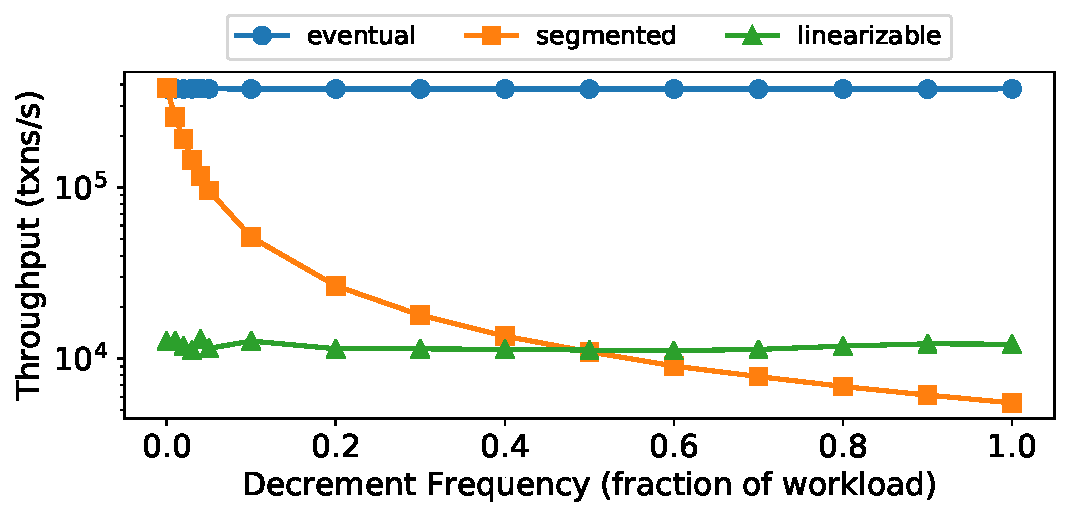
\includegraphics[width=\columnwidth]{figures/throughput_vs_fraction_16.pdf}
  \caption{%
    Segmented \invariantconfluent{} replication throughput versus coordination
    induced by executing disallowed decrement transactions.
  }\figlabel{ThroughputVsGlobalSyncs}
\end{figure}

\begin{benchmark}\benchlabel{VaryWithdraws}
  Consider again the PN-Counter from \exampleref{CounreachableExample} and the
  corresponding transactions, invariants, and single-segment segmentation that
  forbids concurrent decrements. We replicate this object on 16 servers
  deployed on 16 m5.xlarge EC2 instances within the same availability zone.
  Each server has three colocated clients that issue increment and decrement
  transactions. We replicate the object with eventual consistency, segmented
  \invariantconfluence{}, and linearizability and measure the system's total
  throughput as we vary the fraction of client requests that are decrements.
  The results are shown in \figref{ThroughputVsGlobalSyncs}.

  Both eventually consistent replication and linearizable replication are
  unaffected by the workload, achieving roughly 375,000 and 12,000 transactions
  per second respectively. Segmented \invariantconfluent{} replication performs
  well for low-decrement (i.e.\ low-coordination) workloads and performs
  increasingly poorly as we increase the fraction of decrement transactions,
  eventually performing worse than linearizable replication. For example, with
  5\% decrement transactions, segmented \invariantconfluent{} replication
  performs over an order of magnitude better than linearizable replication;
  with 50\% decrements, it performs as well; and with 100\% decrements, it
  performs two times worse.

  % These results are expected. Increment transactions can execute without any
  % coordination while decrement transactions require global coordination. As we
  % increase the fraction of decrements, we increase the amount of coordination
  % that the system has to perform which in turn drastically decreases the
  % throughput. For high contention workloads, segmented \invariantconfluent{} replication performs worse than linearizable replication

  These results offer two insights.
  %
  First, the relationship between segmented \invariantconfluent{} and
  linearizable replication is analogous to the relationship between optimistic
  and pessimistic concurrency control protocols with coordination playing the
  role of contention \jmh{I didn't understand that last clause about ``coordination playing the role of contention.} Linearizable replication pessimistically assumes that
  concurrently executing \emph{any} pair of transactions will lead to an
  invariant violation. Thus, clients send transactions directly to a leader to
  be linearized. Conversely, segmented \invariantconfluent{} replication
  optimistically attempts to perform every transaction locally and without
  coordination. A server only initiates a round of coordination if it is found
  to be necessary. As a consequence, segmented \invariantconfluent{}
  replication can offer substantial performance benefits over linearizable
  replication for low-coordination workloads, but is inferior for medium to
  high contention workloads. \jmh{say why}

  Second, throughput does not decrease linearly with the amount of
  coordination. Even infrequent coordination can drastically decrease
  throughput. Increasing the fraction of decrements from 0\% to 1\% decreases
  throughput by a factor of 2. Increasing again to 3\%, the throughput
  decreases by another factor of 2. With 90\% coordination-free transactions
  (i.e.\ 10\% decrements), we achieve only 10\% of the throughput of eventually
  consistent replication.

%  %
%  First, for low-decrement workloads, segmented \invariantconfluent{}
%  replication achieves a compromise between strong and weak consistency. It
%  guarantees that invariants are maintained (which is impossible with eventual
%  consistency if the object is not \invariantconfluent{}) with performance many
%  times better than strongly consistent replication.
%  %
%  Second, segmented \invariantconfluent{} replication is poorly suited to
%  workloads that require a large amount of coordination. For workloads without
%  much inherit concurrency (e.g.\ decrement-mostly workloads), maintaining
%  invariants is best done with strong consistency. It provides stronger
%  guarantees with better performance.
\end{benchmark}

% \begin{benchmark}\benchlabel{VarySegmentLength}
%   Consider again the object, transactions, and invariants from \exampleref{Z2}
%   and \exampleref{SegmentedZ2}. As with \benchref{VaryWithdraws}, we replicate
%   the object across 32 servers. Clients issue 50\% increment $x$ transactions,
%   and 50\% decrement $y$ transactions. We consider a ``checkerboard''
%   segmentation $\Sigma_n = \setst{(I_{i, j}, T)}{i, j \in \ints}$ where segment
%   invariant $I_{i, j}$ consists of the square of points $\setst{(x, y)}{ni \leq
%   x < n(i + 1), nj \leq y < n(j + 1)}$ with side length $n$. For example,
%   $\Sigma_1$ places each point in its own segment, $\Sigma_2$ tessellates
%   $\ints^2$ with 2x2 squares, $\Sigma_3$ tessellates $\ints^2$ with 3x3
%   squares, and so on. We measure the throughput of the object replicated with
%   eventually consistent, segmented \invariantconfluent{}, and linearizable
%   replication as we vary the segment side length $n$. The results are shown in
%   the bottom \figref{ThroughputVsGlobalSyncs}.
%
%   This benchmark tells the same tale as \benchref{VaryWithdraws}. Eventual
%   consistency and linearizability are unaffected by workload, and eventual
%   consistency outperforms linearizability by roughly two orders of magnitude.
%   In this example, the segmented \invariantconfluent{} replication only
%   requires coordination when transitioning between segment boundaries, so as we
%   increase the segment side length, the throughput of the system increases
%   significantly.
% \end{benchmark}

\begin{figure}[t]
  \centering
  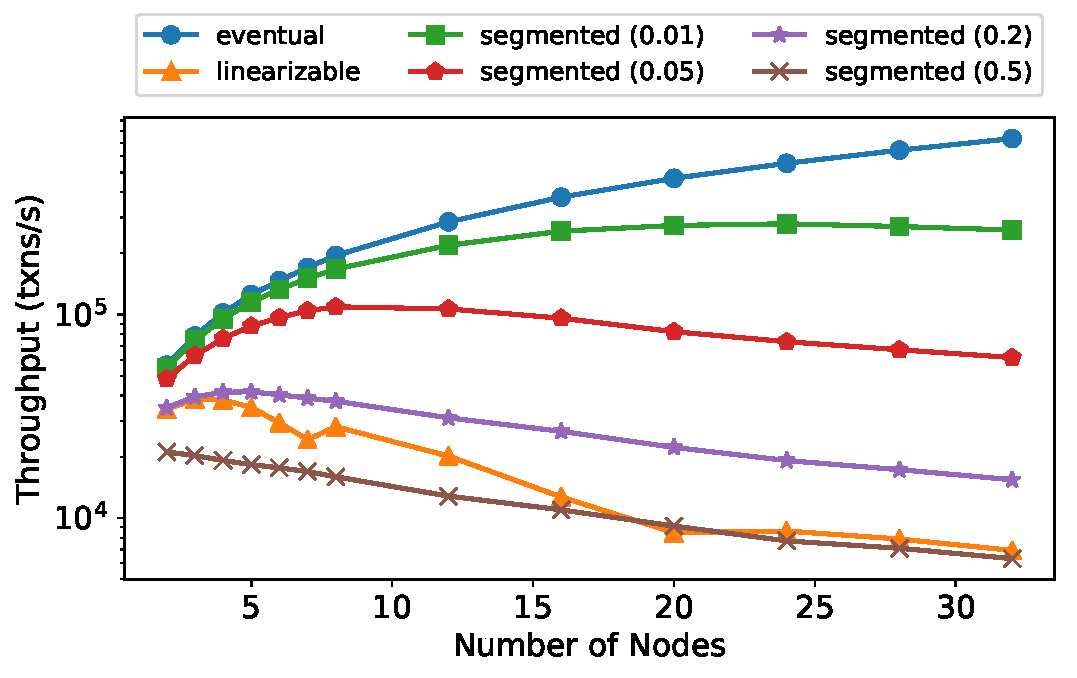
\includegraphics[width=\columnwidth]{figures/throughput_vs_num_nodes_multi.pdf}
  \caption{%
    Throughput of eventually consistent, segmented \invariantconfluent{}, and
    linearizable replication measured against the number of nodes for workloads
    with varying fractions of decrement transactions. For example, the
    ``segmented (0.2)'' line measures the performance of segmented
    \invariantconfluent{} replication with 20\% decrement transactions.
    Eventually consistent replication and linearizable replication are not
    affected by workload.
  }\figlabel{VaryNodes}
\end{figure}

\begin{benchmark}
\jmh{Can you get the figures to color ``eventual'' and ``linearizable'' the same in both?}
  In this benchmark, we measure the scale-out of segmented
  \invariantconfluent{} replication. We repeat \benchref{VaryWithdraws} while
  we vary the number of servers that we use to replicate our object. When we
  replicate with $n$ servers, we use $3n$ clients (the $3$ colocated clients on
  each server) as part of the workload. The results are shown in
  \figref{VaryNodes}.

  Eventually consistent replication scales perfectly with the number of nodes,
  confirming the results in~\cite{bailis2014coordination}. Linearizable
  replication, on the other hand, scales up to about 3 servers before
  performance begins to decrease. Segmented \invariantconfluent{} replication
  scales well for low-coordination workloads and poorly for high-coordination
  workloads. For 1\%, 5\%, 20\%, and 50\% decrement transactions, segmented
  \invariantconfluent{} replication scales up to 24, 12, 4, and 1 server
  respectively.

  These results echo the results of \benchref{VaryWithdraws}. For
  low-coordination workloads, segmented \invariantconfluent{} replication can
  offer almost an order of magnitude better scalability compared to
  linearizable replication, but coordination decreases scalability
  superlinearly. Even infrequent coordination can drastically reduce the
  scalability of segmented \invariantconfluent{} replication with segmented
  \invariantconfluent{} replication ultimately scaling worse than linearizable
  replication for high-coordination workloads.
\end{benchmark}
